\documentclass[11pt]{article}
\usepackage{multicol,pifont,verbatim,fancyvrb,calc,xcolor,xspace}
\usepackage{amsmath, amssymb}
\usepackage{wrapfig,paralist,rotating,subfig}
\usepackage[textwidth=6in,textheight=8in]{geometry}
\usepackage{url}
\usepackage{float}
\usepackage{minted}
\usepackage{xcolor}
\usepackage{hyperref}

% Please use vector graphics in .pdf format where possible
% This is much preferable to large bitmap files
\DeclareGraphicsExtensions{{.pdf},{.jpg},{.png}}

% Definitions ************************************************************

% Some convenient definitions. You may use them or ignore them,
% but I find the ability to extend LaTeX to be enormously useful.

% To refer to an equation, use \eref{<label>}, where <label> is the
% part that follows the 'eq:' in the label of the equation.
\newcommand{\eref}[2][]{%
	\ifthenelse{\equal{#1}{}}%
	{Eq.~(\ref{eq:#2})}%
	{Equation~(\ref{eq:#2})}\xspace}

% To refer to a figure, use \fref{<label>}, where <label> is the
% part that follows the 'fig:' in the label of the figure.
\newcommand{\fref}[2][]{%
  \ifthenelse{\equal{#1}{}}%
	{Fig.~\ref{fig:#2}}%
	{Figure~\ref{fig:#2}}}

% How to type vectors. If you don't like this style, you can just change
% the definition of \VEC!!
\newcommand{\VEC}[1]{\ensuremath{\boldsymbol{#1}}\xspace}

% unit vectors
\newcommand{\ux}{\ensuremath{\mathbf{\hat{x}}}\xspace}
\newcommand{\uy}{\ensuremath{\mathbf{\hat{x}}}\xspace}
\newcommand{\uz}{\ensuremath{\mathbf{\hat{x}}}\xspace}

% theta dot and double dot
\newcommand{\thd}{\ensuremath{\dot{\theta}}\xspace}
\newcommand{\thdd}{\ensuremath{\ddot{\theta}}\xspace}

% Derivatives. Some publications require the d in a differential
% to be set in roman. I've never liked that, but I have trained myself
% always to use these two macros, so if I need to switch, it is
% painless.
\newcommand{\DD}{\ensuremath{d}}		% differential d without leading space
\newcommand{\dd}{\ensuremath{\,\DD}}	% differential d

% A normal (total) derivative. If you supply an optional argument n,
% then you get the nth derivative: e.g., \deriv[2]{x}{t}
\newcommand{\deriv}[3][]{\ensuremath{%
	\ifthenelse{\equal{#1}{}}{\frac{\DD #2}{\DD #3}}
	{\frac{\DD^{#1} #2}{\DD #3^{#1}}}}}

% partial derivative
\newcommand{\pd}[3][]{\ensuremath{%
	\ifthenelse{\equal{#1}{}}{\frac{\partial #2}{\partial #3}}
	{\partial #2 / \partial #3}}}

% variational derivative
\newcommand{\varder}[2][]{\ensuremath{\deriv{}{t} \left( \pd{L}{\dot{#2}%
      \ifthenelse{\equal{}{#1}}{}{_{#1}}} \right)} - \pd{L}{#2%
      \ifthenelse{\equal{}{#1}}{}{_{#1}}} }


% Beginning of the settings you need to modify ****************************************




\title{Planar Circular-Restricted 3-Body Problem}
\author{Kavi and Maya}
\date{December 16, 2024}

\begin{document}

\maketitle

\section{Introduction}

% \begin{figure}[b!]
% 	\centering
%     % \includegraphics[width=1.75in]{figs/samplefig.pdf}
% 	\caption{Make the caption informative. Note that this figure does
%       not really represent the system described in the text!}
% 	\label{fig:samplefig}
% \end{figure}


\begin{figure}[H]
    \centering
    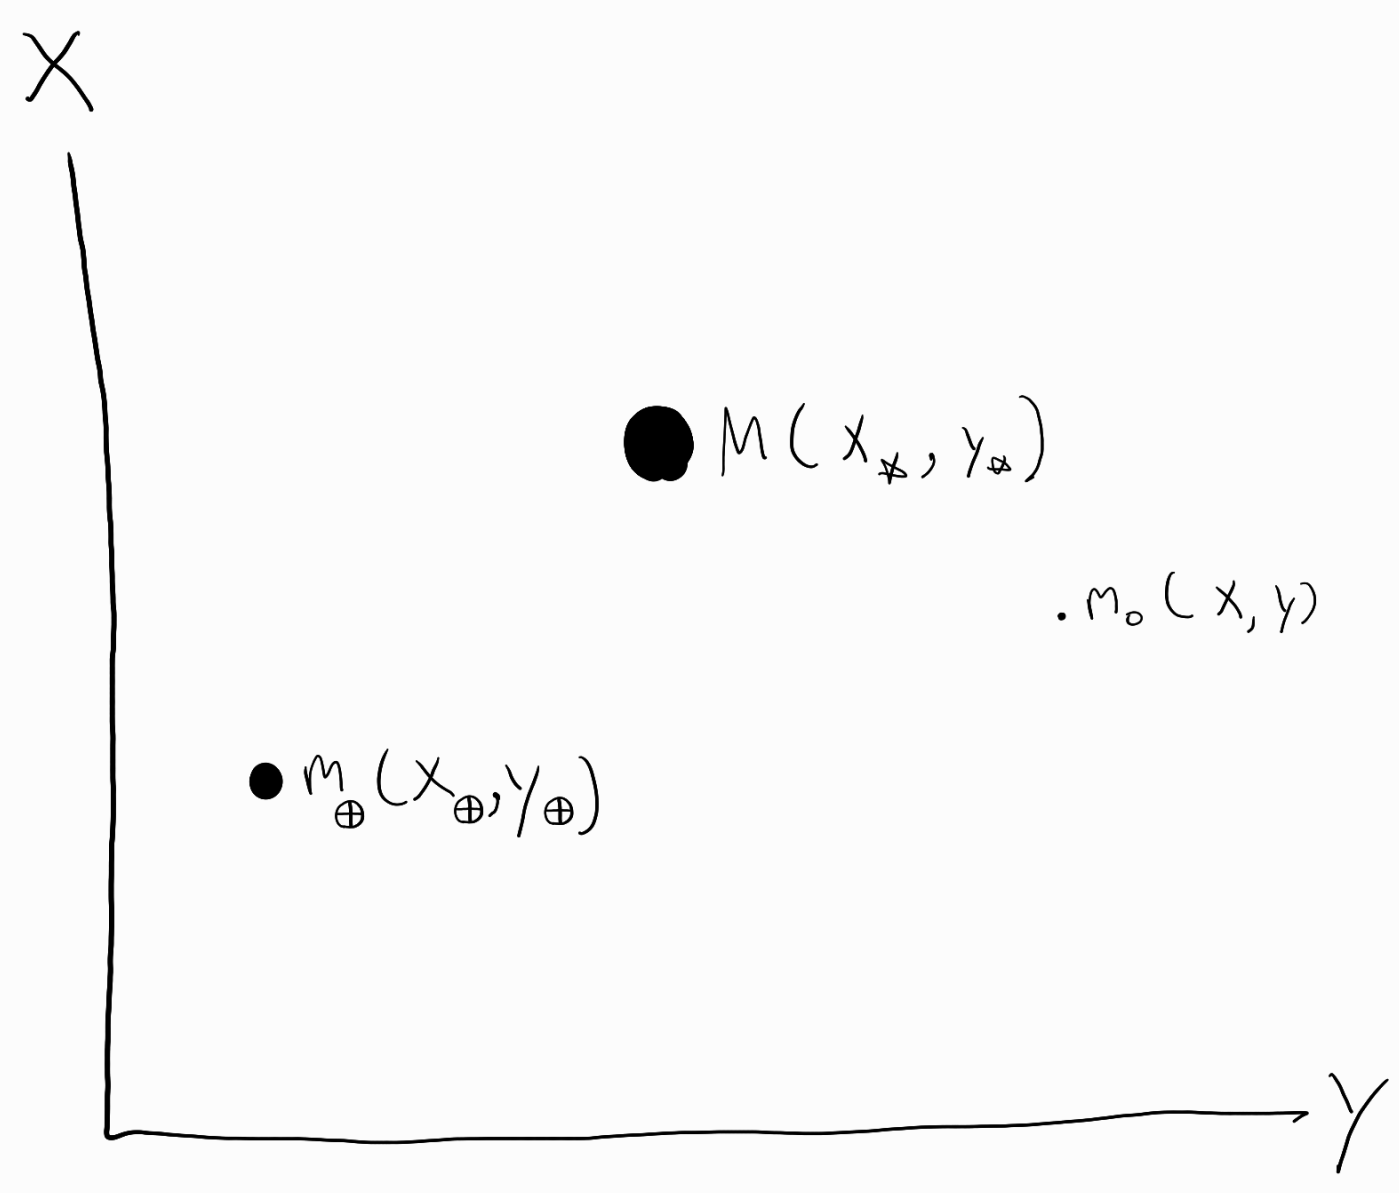
\includegraphics[width=0.5\linewidth]{figures/3body.png}
    \caption{Our three-body system (not to scale)}
    \label{fig:3body}
\end{figure}
  
In this project, we are investigating the dynamics of the planar restricted three body problem. The system consists of three bodies: a star of mass $M$, planet of mass $m_\oplus$, and an asteroid of mass $m_{0}$. We imagine all motion to be constrained to lie in a plane, with all forces along that plane and arising only between the gravitational interactions between the 3 bodies. To make the famously unsolveable 3-body problem a more tractable one, we restrict it to have the planet orbit circularly around the star. 
\\
\\
\noindent
As \href{https://orbital-mechanics.space/the-n-body-problem/circular-restricted-three-body-problem.html}{Bryan Weber} pointed out, this feels like a lot of restrictions, but the planar-restricted 3-body problem actually applies to a fair number of systems that we care about. For example, the earth's orbit around the sun is almost circular (with an eccentricity of 0.017)! Thus, from here on out, we'll refer to the planet as the earth. 
\\
\\
\noindent
That said, just so long as the orbit's circular, it need not be restricted with earth being the only planet; you could also use, say, venus (with an eccentricity of \href{https://nssdc.gsfc.nasa.gov/planetary/factsheet/venusfact.html}{0.007}).
\\
\\
\noindent
This restriction also makes kinetic and potential energies of the earth and sun part both constant, which simplifies the math.
% Then, we can see how different distances between each of the bodies can change the asteroid's motion!
Furthermore, we can see how slight differences in the asteroid's starting position and velocities impact its trajectory! 

\section{Derivation of Lagrangian and Equations of Motion}
% \begin{figure}
%     \centering
%     \includegraphics[width=0.5\linewidth]{figures/3_body_relative.png} 
%     \caption{Caption}
%     \label{fig:3-body-relative}
% \end{figure}

We make the simplifying assumption that the asteroid's mass is significantly less than the other two, such that it does not affect their orbits. This means that we can use the solutions of the two body problem, where the sun and the earth both have perfectly circular orbits of frequency $\Omega$ and radius $a$ around the center of mass of the system. Using Cartesian coordinates to tackle the problem, and we have: 
\begin{align}
    x_\star &= -fa\cos\Omega t \\
    y_\star &= -fa\sin\Omega t \\
    x_\oplus &= (1-f)a\cos\Omega t \\
    y_\oplus &= (1-f)a\sin\Omega t \\
\end{align}
Where ($x_\star, y_\star$) is the position of the sun ($M$) and ($x_\oplus, y_\oplus$) is the position of earth ($m$). We define ($x, y$) as the position of the asteroid ($m_0$). $f$ is defined as a mass ratio that is the earth:
\begin{equation}
    f = \frac{m_\oplus}{M+m_\oplus}
\end{equation}
and $1-f$ is the mass ratio that is the sun:
\begin{equation}
    1-f = \frac{M}{M+m_\oplus}
\end{equation}
\noindent
Then, we define the kinetic and potential energies as follows:
\begin{align}
    T &= \underbrace{\frac{1}{2}m_{0} (\dot x ^2 + \dot y ^2)}_\text{asteroid kinetic energy} + \underbrace{\frac{1}{2}\mu \Omega^{2} a^{2}}_\text{sun-earth kinetic energy} \\
    U &= \underbrace{\frac{Gm_\oplus M}{a}}_\text{sun-earth potential energy} + \underbrace{\frac{G M m_{0}}{\sqrt{(x+fa\cos(\Omega t))^2 +(y+fa\sin(\Omega t))^2}}}_\text{sun-asteroid potential energy} \nonumber \\
    & \quad +\underbrace{\frac{G m_\oplus m_{0}}{\sqrt{(x+(f-1)a\cos(\Omega t))^2 +(y+(f-1)a\sin(\Omega t))^2}}}_\text{earth-asteroid potential energy}
\end{align}
% \begin{align}
% L &= \frac{G M m_{0}}{\sqrt{\left(a f \sin{\left(\tau \right)}+ y{\left(t \right)}\right)^{2} + \left(a f \cos{\left(\tau \right)} + x{\left(t \right)}\right)^{2}}} \nonumber \\
%   & \quad + \frac{G M_{s} m_{e}}{\sqrt{\left(- a \left(1 - f\right) \sin{\left(\tau \right)} + y{\left(t \right)}\right)^{2} + \left(- a \left(1 - f\right) \cos{\left(\tau \right)} + x{\left(t \right)}\right)^{2}}} \nonumber \\
%   & \quad + \frac{G M_{s} m_{e}}{a} + 0.5 \Omega^{2} \mu a^{2} + 0.5 m_{a} \left(\left(\frac{d}{d t} x{\left(t \right)}\right)^{2} + \left(\frac{d}{d t} y{\left(t \right)}\right)^{2}\right)
% \end{align}
where $\mu\ = \frac{Mm_\oplus}{M+m_\oplus}$ is the reduced mass of the earth and the sun. Unfortunately, since the coordinates we're using involve a time transformation from Cartesian coordinates, the Hamiltonian is not the total energy. Moreover, the Hamiltonian is not conserved, since we can see that $\frac{\partial L}{\partial t}\neq0$.
% However, we currently have 4 degrees of freedom $(x,\dot x, y, \dot y)$ and want only one degree of freedom. So, we want the Hamiltonian to be conserved so we can use it to take away a degree of freedom! So,
However, By using a time-dependent coordinate transform we can jump onto the rotating sun-earth frame, eliminating the dependence on $t$ and making $H$ conserved (note that $H\neq T+U$). We will apply the following transform to get $x',y'$, the position of the asteroid in the rotating frame:

\begin{figure}[H]
    \centering
    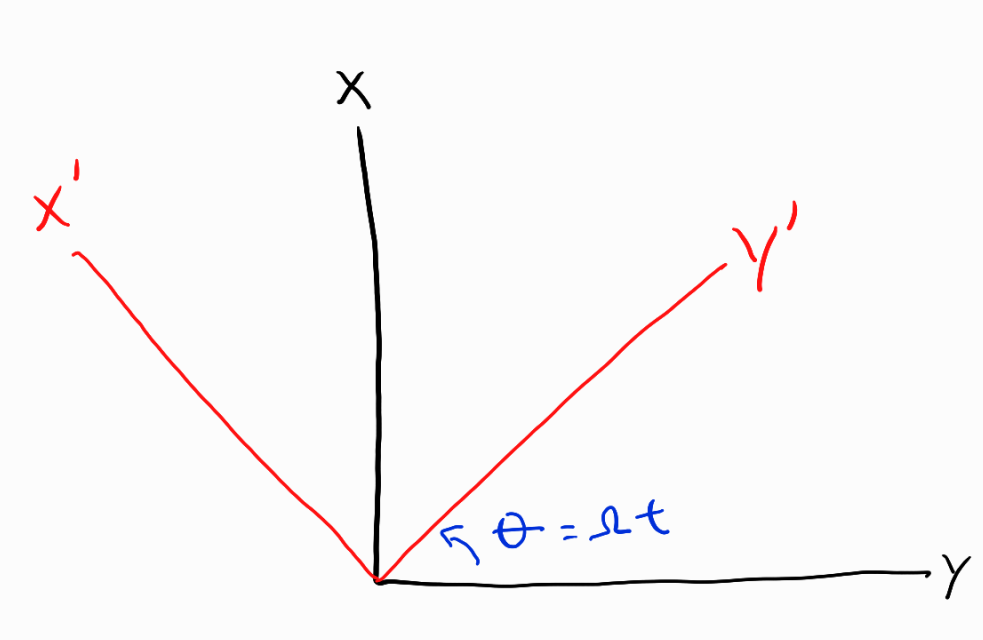
\includegraphics[width=0.5\linewidth]{figures/coord_transform2.png}
    \caption{Coordinate transform to frame where sun and earth are stationary}
    \label{fig:coord_transform2}
\end{figure}

% \begin{figure}
%     \centering
%     \includegraphics[width=0.5\linewidth]{figures/coord_transform.png}
%     \caption{Coordinate transform to frame where sun and earth are stationary}
%     \label{fig:coord_transform}
% \end{figure}

\begin{equation}
    \begin{bmatrix}
        x \\ y
    \end{bmatrix}
    =
    \begin{bmatrix}
        \cos\theta & -\sin\theta \\
        \sin\theta & \cos\theta
    \end{bmatrix}
    \begin{bmatrix}
        x'\\y'
    \end{bmatrix}
\end{equation}
Evaluating this we get:
\begin{align}
    x &= x'\cos \Omega t - y'\sin \Omega t \\
    \dot x &= \dot x' \cos\Omega t - \dot y'\sin\Omega t - x'\Omega\sin\Omega t - y'\Omega\cos\Omega t \\
    y &= x'\sin\Omega t + y'\cos\Omega t \\
    \dot y &= \dot x' \sin\Omega t + \dot y'\cos\Omega t + x'\Omega\cos\Omega t - y'\Omega\sin\Omega t
\end{align}
\noindent
Now we can substitute this into the kinetic energy term of the old Lagrangian to get a new kinetic energy term $T'_{m_{0}}$ for the mass $m_{0}$ with:

\begin{align*}
    T_{\dot x, \text{squared terms}} & = \frac{1}{2}m_{0}(\dot x'^2 \cos^2 \Omega t + \dot y'^2\sin^2\Omega t + x'^2\Omega^2\sin^2\Omega t + y'^2\Omega^2\cos^2\Omega t)\\
    T_{\dot y, \text{squared terms}} & =\frac{1}{2}m_{0}(\dot x'^2\sin^2\Omega t + \dot y'^2\cos^2\Omega t + x'^2\Omega^2\cos^2\Omega t + y'^2\Omega^2\sin^2\Omega t) \\
    T_{\dot x, \text{cross terms}} & = \frac{1}{2}m_{0}(-\underbrace{2\dot x'\dot y'\sin\Omega t\cos\Omega t}_{a} - \underbrace{2\dot x'x'\Omega\sin\Omega t\cos\Omega t}_{b}-2\dot x' y'\Omega\cos^2\Omega t \\
    & \quad + 2x'\dot y' \Omega\sin^2\Omega t + \underbrace{2y'\dot y'\Omega\sin\Omega t\cos\Omega t}_{c} + \underbrace{2x'y'\Omega^2\sin\Omega t\cos\Omega t}_{d})\\
    T_{\dot y, \text{cross terms}} & = \frac{1}{2}m_{0}(\underbrace{2\dot x'\dot y'\sin\Omega t\cos\Omega t}_a + \underbrace{2\dot x'x'\Omega\sin\Omega t\cos\Omega t}_{b} - 2\dot x'y'\Omega \sin^2\Omega t \\
    & \quad + 2x'\dot y'\Omega\cos^2 t - \underbrace{2y'\dot y'\Omega\sin\Omega t\cos\Omega t}_{c} - \underbrace{2x'y'\Omega^2\sin\Omega t\cos\Omega t}_{d})
\end{align*}
When these four equations are added together to get $T'_{m_{0}}$, terms $a,b,c,\text{and }d$ cancel out, leaving us with

\begin{align}
    \hspace{-5cm}T' &= \frac{1}{2}\mu a^2\Omega^2 + T'_{m_{0}} \\
    &= \frac{1}{2}\mu a^2\Omega^2 + \frac{1}{2}m_0(\dot x'^2 +\dot y'^2) + \frac{1}{2}m_0\Omega^2(x'^2 + y'^2) + m_0\Omega(x'\dot y' - \dot x' y')
\end{align}

Now we can write the system Lagrangian in the rotating frame as:
\begin{align}
    L &= \underbrace{\frac{1}{2}\mu_{\star\oplus}a^2\Omega^2}_\text{constant, ignored} + \frac{1}{2}m_0(\dot x'^2 +\dot y'^2) + \underbrace{\frac{1}{2}m_0\Omega^2(x'^2 + y'^2)}_\text{centrifugal force} + \underbrace{m_0\Omega(x'\dot y' - \dot x' y')}_\text{coriolis force} \nonumber \\
    & \quad + \underbrace{\frac{GMm_\oplus}{a}}_\text{constant, ignored} + \frac{GMm_0}{r_\star} + \frac{Gm_\oplus m_0}{r_\oplus}
\end{align}

Where
\begin{align}
    r_\star &= \sqrt{(x'+fa)^2 + y'^2} \\
    r_\oplus &= \sqrt{(x'-(1-f)a)^2 + y'^2}
\end{align}

From the Lagrangian, we can now derive the Hamiltonian as
\begin{align}
    H &= (\sum q_i\frac{\partial L}{\partial q_i}) - L \\ 
    \frac{\partial L}{\partial \dot x'} &= m\dot x' -m\Omega y' \\
    \frac{\partial L}{\partial \dot y'} &= m\dot y' + m\Omega x' 
\end{align}
Writing out the full Hamiltonian we get:
\begin{align}
    H &= m\dot x'^2 - \underbrace{m\Omega y'\dot x'}_a + m\dot y'^2 + \underbrace{m\Omega x'\dot y'}_b - \frac{1}{2}m(\dot x'^2 + \dot y'^2) - \frac{1}{2} m\Omega^2(x'^2 + y'^2) \nonumber \\
    & \quad - m\Omega(\underbrace{x'\dot y'}_b - \underbrace{\dot x' y'}_a) - \frac{GMm_{0}}{r_\star} - \frac{Gm_\oplus m_{0}}{r_\oplus}
\end{align}
then canceling out the $a$ and $b$ terms we get
\begin{equation}
    H = \frac{1}{2}m_{0}(\dot x'^2 + \dot y'^2) - \frac{1}{2} m_{0}\Omega^2(x'^2 + y'^2)  - \frac{GMm_{0}}{r_\star} - \frac{Gm_\oplus m_{0}}{r_\oplus}
\end{equation}
Note that after the coordinate transform, $H$ is conserved, so we can use it to help set initial conditions and reason about the problem. %eliminate one of the four degrees of freedom.

\section{Euler-Lagrange Equations}
Computing our Euler-Lagrange equations (using python) for $x'$ we get:
\begin{align}
        \frac{\partial L}{\partial x'} &=\Omega m_{0} \dot y' 
        +\Omega ^2 m_{0} x' -\frac{Gm_\oplus m_{0}(x'+af-a)}{[(x'+af-a)^2 +(y')^2]^{3/2}}-\frac{GM m_{0}(x'+af)}{[(x'+af)^2 +(y')^2]^{3/2}} \\
        \dfrac{d}{dt}\left(\frac{\partial L}{\partial \dot x'}\right) &=-\Omega m_{0} \dot y' 
        + m_{0}\ddot x' \\
        -\Omega m_{0} \dot y' + m_{0}\ddot x' &=\Omega m_{0} \dot y' 
        +\Omega ^2 m_{0} x' -\frac{Gm_\oplus m_{0}(x'+af-a)}{[(x'+af-a)^2 +(y')^2]^{3/2}}-\frac{GM m_{0}(x'+af)}{[(x'+af)^2 +(y')^2]^{3/2}}
\end{align}
And, for $y'$
\begin{align}
        \frac{\partial L}{\partial y'} &=-\Omega m_{0} \dot x' 
        +\Omega ^2 m_{0} y' -\frac{Gm_\oplus m_{0}y'}{[(x'+af-a)^2 +(y')^2]^{3/2}}-\frac{GM m_{0}y'}{[(x'+af)^2 +(y')^2]^{3/2}} \\
        \dfrac{d}{dt}(\frac{\partial L}{\partial \dot y'}) &=\Omega m_{0} \dot x' 
        + m_{0}\ddot y' \\
        \Omega m_{0} \dot x' 
        + m_{0}\ddot y' &=-\Omega m_{0} \dot x' 
        +\Omega ^2 m_{0} y' -\frac{Gm_\oplus m_{0}y'}{[(x'+af-a)^2 +(y')^2]^{3/2}}-\frac{GM m_{0}y'}{[(x'+af)^2 +(y')^2]^{3/2}}
\end{align}
Now, we use Python to solve both of these equations to isolate the second derivatives to get our equations of motion.
\begin{align}
    \ddot  x' &= 2 \Omega \dot y' +\Omega ^2 x' - \frac{Gm_\oplus (x'-a+af)}{[(af-a+x')^2 +(y') ^2]^{3/2}} -\frac{GM (x'+af)}{[(af+x')^2 +(y') ^2]^{3/2}}
\end{align}

\begin{align}
    \ddot  y' &= -2 \Omega \dot x' +\Omega ^2 y' - \frac{Gm_\oplus y}{[(af-a+x')^2 +(y') ^2]^{3/2}} -\frac{GM y}{[(af+x')^2 +(y') ^2]^{3/2}}
\end{align}



\section{Nondimensionalization}

Now, we nondimensionalize our Euler-Lagrange equations and Hamiltonian. First let we use the orbital period from the two body problem a characteristic time via
\begin{equation}
    t=T_0\tau, \quad T_0=1/\Omega
\end{equation}
where $T_0$ has units of seconds.
Substituting this in, we get
\begin{align}
    \Omega^2 \frac{\partial^2 x'}{\partial \tau^2}
    =2 \Omega^2 \frac{\partial y'}{\partial \tau}
    +\Omega ^2 x' - \frac{Gm_\oplus (x'-a+af)}{[(af-a+x')^2 +(y') ^2]^{3/2}} -\frac{GM (x'+af)}{[(af+x')^2 +(y') ^2]^{3/2}}
\end{align}
\begin{align}
    \Omega^2 \frac{\partial^2 y'}{\partial \tau^2}
    =-2 \Omega^2 \frac{\partial x'}{\partial \tau}
    +\Omega ^2 y' - \frac{Gm_\oplus y'}{[(af-a+x')^2 +(y') ^2]^{3/2}} -\frac{GM y'}{[(af+x')^2 +(y') ^2]^{3/2}}
\end{align}
\begin{equation}
    H = \frac{1}{2}m_{0}(\Omega^2 (\frac{\partial x'}{\partial \tau})^2 + \Omega^2 (\frac{\partial y'}{\partial \tau})^2 - \frac{1}{2} m_{0}\Omega^2(x'^2 + y'^2)  - \frac{GMm_{0}}{\sqrt{(x'+fa)^2 + y'^2}} - \frac{Gm_\oplus m_{0}}{\sqrt{(x'-(1-f)a)^2 + y'^2)}}
\end{equation}
Next we non-dimenstionalize the position of $m_0$ based off of the distance $a$ between $M$ and $m_\oplus$
\begin{equation}
    X'=x'/a
\end{equation}
\begin{equation}
    Y'=y'/a
\end{equation}
Which results in
\begin{align}
    \Omega^2 a \frac{\partial^2 X'}{\partial \tau^2}
    =2 \Omega^2 a\frac{\partial Y'}{\partial \tau}
    +\Omega ^2 aX' - \frac{Gm_\oplus a(X'-1+f)}{[(f-1+X')^2 +(Y') ^2]^{3/2}a^3} -\frac{GM a(X'+f)}{[(f+X')^2 +(Y') ^2]^{3/2}a^3}
\end{align}
\begin{align}
    \Omega^2 a \frac{\partial^2 Y'}{\partial \tau^2}
    =-2 \Omega^2 a\frac{\partial X'}{\partial \tau}
    +\Omega ^2 aY' - \frac{Gm_\oplus aY'}{[(f-1+X')^2 +(Y') ^2]^{3/2}a^3} -\frac{GM aY'}{[(f+X')^2 +(Y') ^2]^{3/2}a^3}
\end{align}
\begin{align}
    H &= \frac{1}{2}m_{0}\left(\Omega^2 a^2 \left(\frac{\partial X'}{\partial \tau}\right)^2 + \Omega^2 a^2 \left(\frac{\partial Y'}{\partial \tau}\right)^2 \right) \nonumber \\
    & \quad - \frac{1}{2} m_{0}\Omega^2 a^2(X'^2 + Y'^2)   - \frac{GMm_{0}}{a\sqrt{(X'+f)^2 + Y'^2}} - \frac{Gm_\oplus m_{0}}{a\sqrt{(X'-(1-f))^2 + Y'^2)}}
\end{align}
Now, we cancel out a factor of $a \Omega^2$ on both sides of the Euler-Lagrange equations:
\begin{align}
    \frac{\partial^2 X'}{\partial \tau^2}
    =2 \frac{\partial Y'}{\partial \tau}
    +X' - \frac{Gm_\oplus (X'-1+f)}{[(f-1+X')^2 +(Y') ^2]^{3/2}a^3\Omega^2} -\frac{GM (X'+f)}{[(f+X')^2 +(Y') ^2]^{3/2}a^3\Omega^2}
\end{align}
\begin{align}
    \frac{\partial^2 Y'}{\partial \tau^2}
    =-2 \frac{\partial X'}{\partial \tau}
    +Y' - \frac{Gm_\oplus Y'}{[(f-1+X')^2 +(Y') ^2]^{3/2}a^3\Omega^2} -\frac{GM Y'}{[(f+X')^2 +(Y') ^2]^{3/2}a^3\Omega^2}
\end{align}
And cancel out a factor of $m_0a^2 \Omega^2$ in the Hamiltonian:
\begin{align}
    \frac{H}{m_{0}a^2 \Omega^2} &= \frac{1}{2}\left( \left(\frac{\partial X'}{\partial \tau}\right)^2 \ +  \left(\frac{\partial Y'}{\partial \tau}\right)^2 \right) - \frac{1}{2} (X^2 + Y'^2) \nonumber \\
    & \quad - \frac{GM}{a^3\Omega ^2\sqrt{(X'+f)^2 + Y'^2}} - \frac{Gm_\oplus }{a^3\Omega ^2\sqrt{(X'-(1-f))^2 + Y'^2)}}
\end{align}
Now, let d, e, and h be dimensionless parameters such that
\begin{align}
    d &= \frac{Gm_\oplus}{\Omega^2 a^3} \\
    e &= \frac{GM}{\Omega^2 a^3} \\
    h &= \frac{H}{m_{0}\Omega^2 a^2}
\end{align}
We then get our fully nondimensionalized equations: 
\begin{align}
    \frac{\partial^2 X'}{\partial \tau^2}
    & =2 \frac{\partial Y'}{\partial \tau}
    +X' - \frac{d (X'-1+f)}{[(f-1+X')^2 +(Y') ^2]^{3/2}} -\frac{e (X+f)}{[(f+X')^2 +(Y') ^2]^{3/2}} \\
    \frac{\partial^2 Y'}{\partial \tau^2}
    & =-2 \frac{\partial X'}{\partial \tau}
    +Y' - \frac{d Y'}{[(f-1+X')^2 +(Y') ^2]^{3/2}} -\frac{e Y}{[(f+X')^2 +(Y') ^2]^{3/2}} \\
    h &= \frac{1}{2}\left( \left(\frac{\partial X'}{\partial \tau}\right)^2 +  \left(\frac{\partial Y'}{\partial \tau}\right)^2 \right) - \frac{1}{2} (X'^2 + Y'^2)   - \frac{e}{\sqrt{(X'+f)^2 + Y'^2}} - \frac{d}{\sqrt{(X'-(1-f))^2 + Y'^2)}}
\end{align}

% \section{Integration}
% \label{sec:Integration}
% Now, we use Python to integrate the equations for $\frac{\partial^2 X}{\partial \tau^2}$ and $\frac{\partial^2 Y}{\partial \tau^2}$, getting (SOMETHING/SHOW PLOT). 

% Then, we graph h, which is the Hamiltonian divided by a bunch of conserved quantities, over $\tau$. $\tau$ is just time off by a factor of $\Omega$, so h should be conserved as we change $\tau$. We get the plot: (ADD PLOT). 


\section{Results}
\label{sec:Results}
\subsection{Circular Orbits}
 We start with an exploration of simple test cases to confirm our equations, with $\Omega=G=M=a=1$ and $m_\oplus=0.1$ for ease of investigation. Note that this results in $d=0.1, e=1.0, f=0.091$. If $M >> m_\oplus$ and $m_0$ is close to either one, the gravitational potential energy of the closer mass should dominate and $m_0$ will orbit around it. With these parameters, testing a few radii and initial velocities of the asteroid, we see the following circular orbits:
\begin{figure}[H]
    \centering
    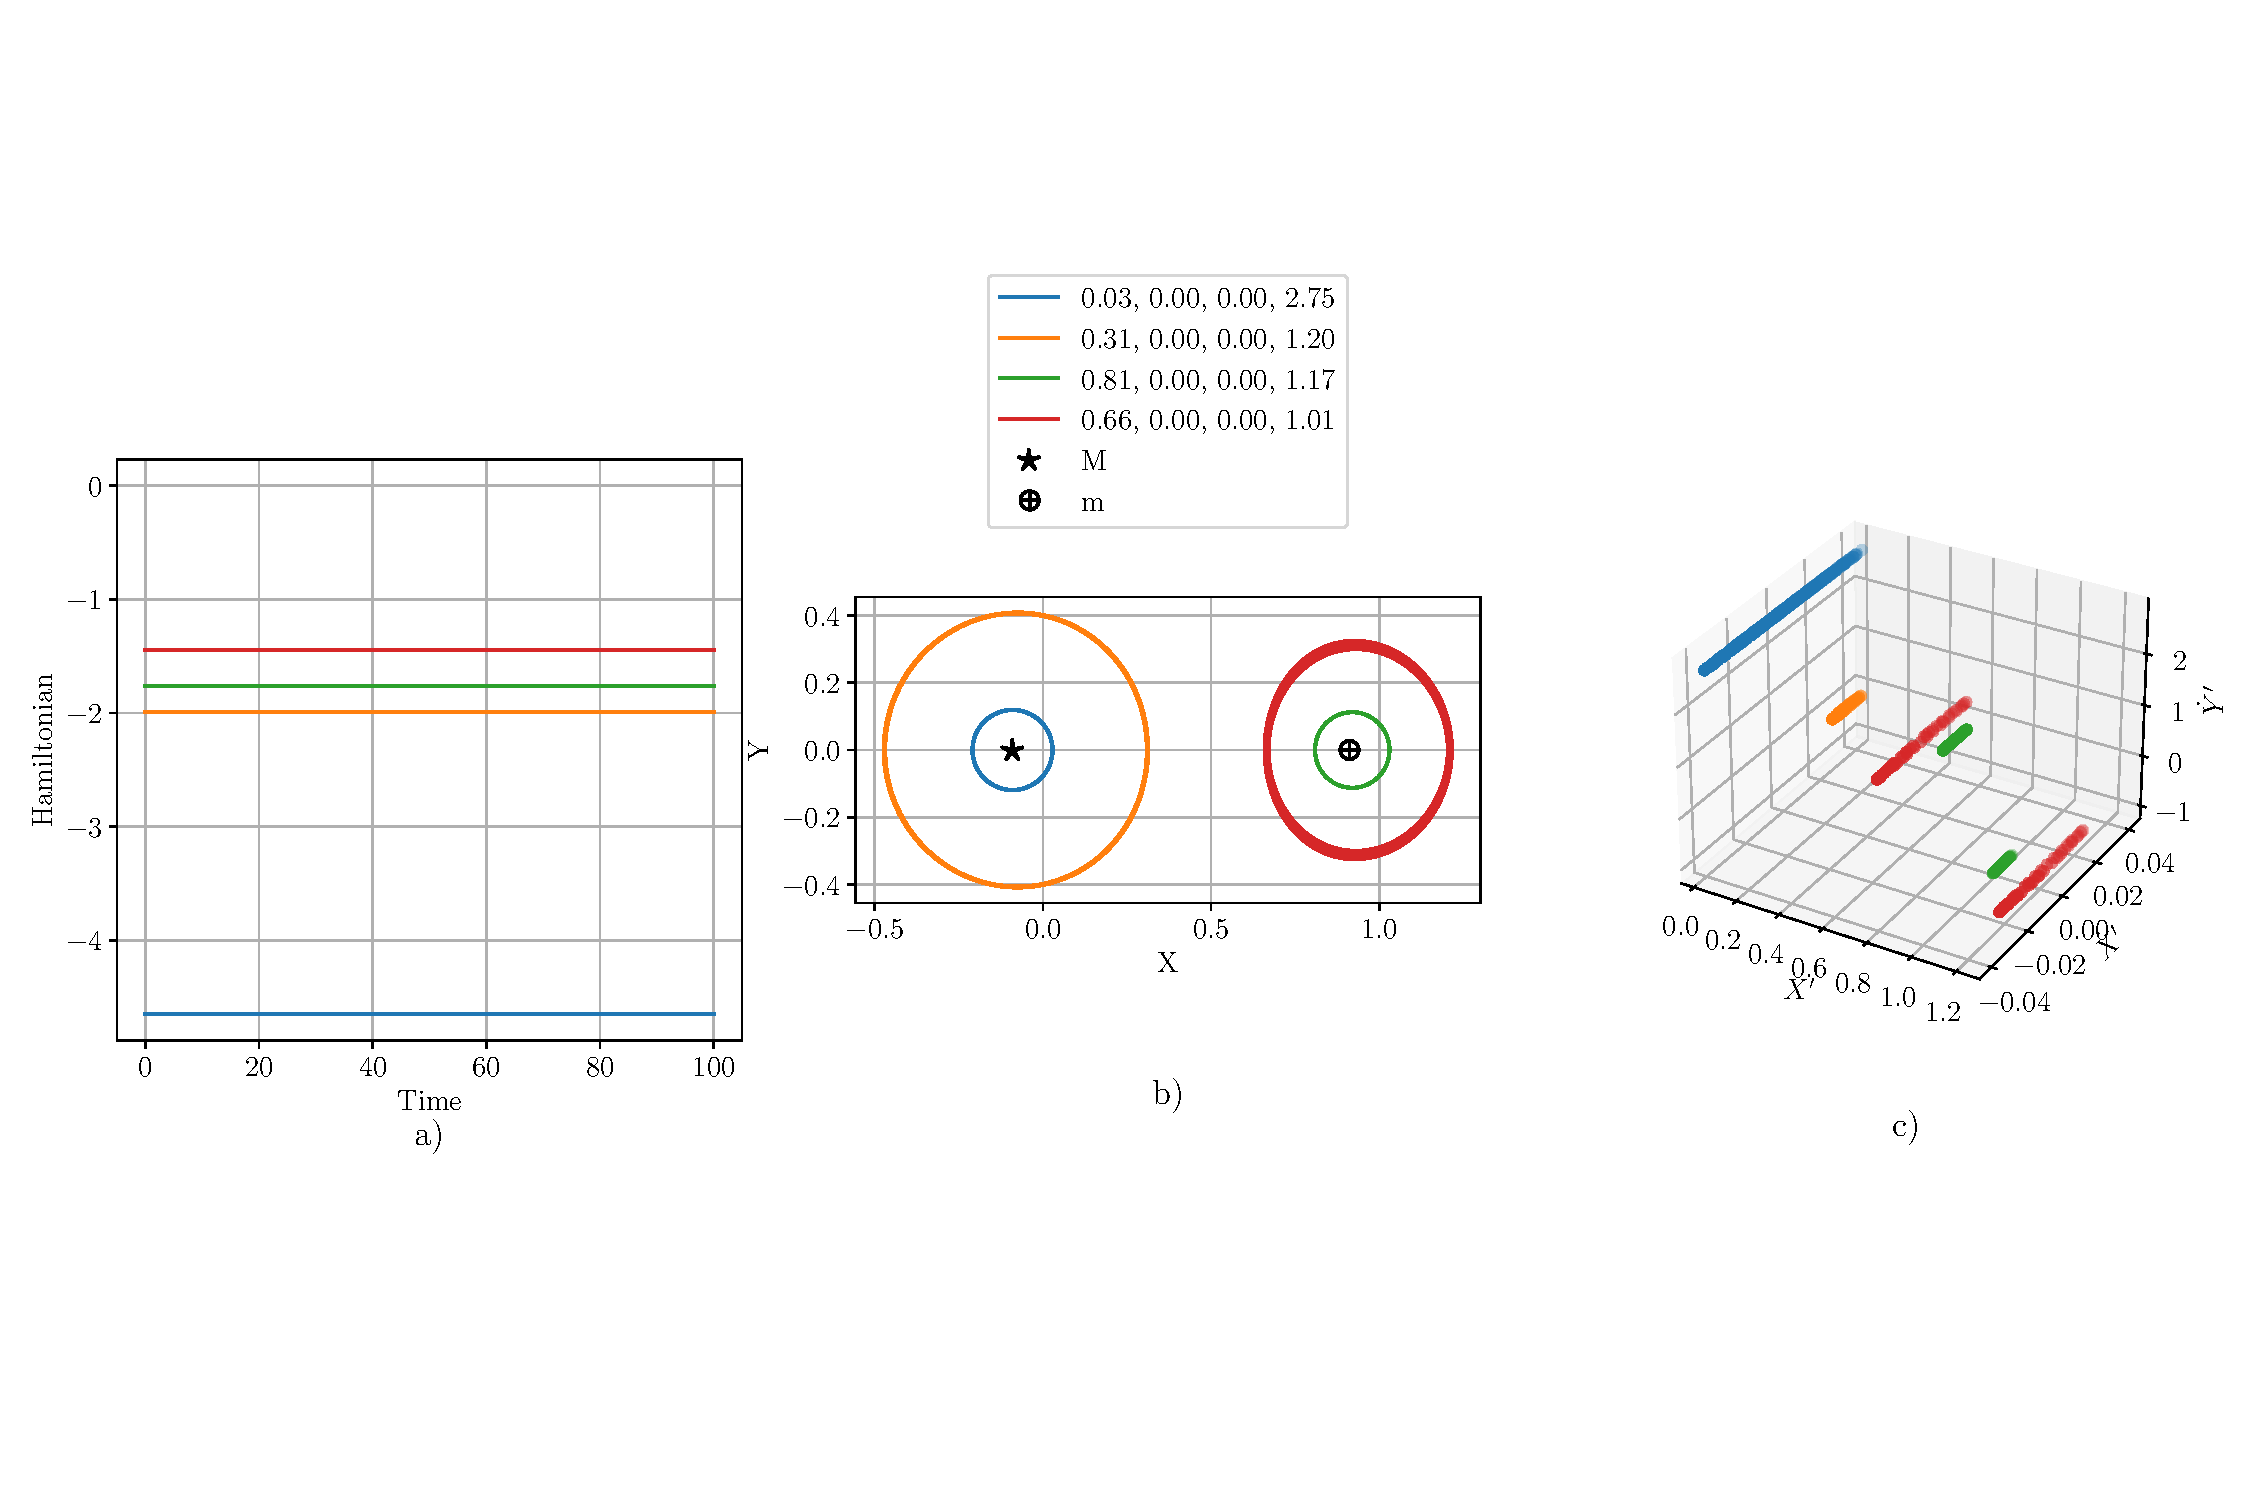
\includegraphics[width=1\linewidth]{figures/circular_orbits.pdf}
    \caption{a) Hamiltonian over time plot of each initial condition to show conservation as predicted. b) Circular trajectories taken by $m_0$ around $M$ and $m_\oplus$. Initial conditions are listed as $(X', \dot X', Y', \dot Y')$. c) Surface of section plotted for $\tau \in (0,1000)$}
    \label{fig:circular-orbits}
\end{figure}
\noindent
For the surface of section, we slice along $Y'=0$ and $X'>0$ plotting $(x,y,z) = (X',\dot X',\dot Y')$. This point was chosen because is when $m_0$ crosses the X'-axis, thus passing between the line formed by $M$ and $m_0$.
It is plotted over a longer time span than the Hamiltonian and $m_0$ trajectories to increase the number of points and create a denser plot. We notice that, for a given $X'$ value, there are a range of possible $\dot Y'$ values, but these are all very close to 0. This makes sense; if the asteroid is orbiting either body, it should only have velocity in the vertical direction when it is passing the X'-axis, so $\dot X'$ should be 0! 
\\
\\
\noindent
\textit{A note on calculating intersection points for the surfaces of section:} \\
To slice along $Y'=0$, we must first determine where that is. However, we cannot do this analytical because we are integrating with respect to $\tau$ and can't do a change of variables to switch to integrating with respect to $X'$ (because $X'$ needs to be able to increase and decrease). Instead, we solve the trajectory with respect to time and numerically determine the crossing point using the following algorithm:
\begin{minted}{python}
Y = [...] # y trajectory
X = [...] # X trajectory

idxs = []
chk = -np.abs(Y)

# Loop through all items in Y
for i in range(1, len(Y)-1):
    # Check if
    # - the current point is a peak (greater than both of its neighbors)
    # - the current point is a peak at 0 (within delta of 0)
    # - the current point has a positive X value
    if (chk[i - 1] < chk[i] > chk[i + 1]) and chk[i] > -0.01 and X[i] > 0:
        idxs.append(i)
\end{minted}
This converts the problem of determining when $-\delta <Y' < \delta$, finding peaks in $|Y'|$ which is much easier to do. Running this for the blue trajectory in Figure \ref{fig:circular-orbits} we get the following plot:
\begin{figure}[H]
    \centering
    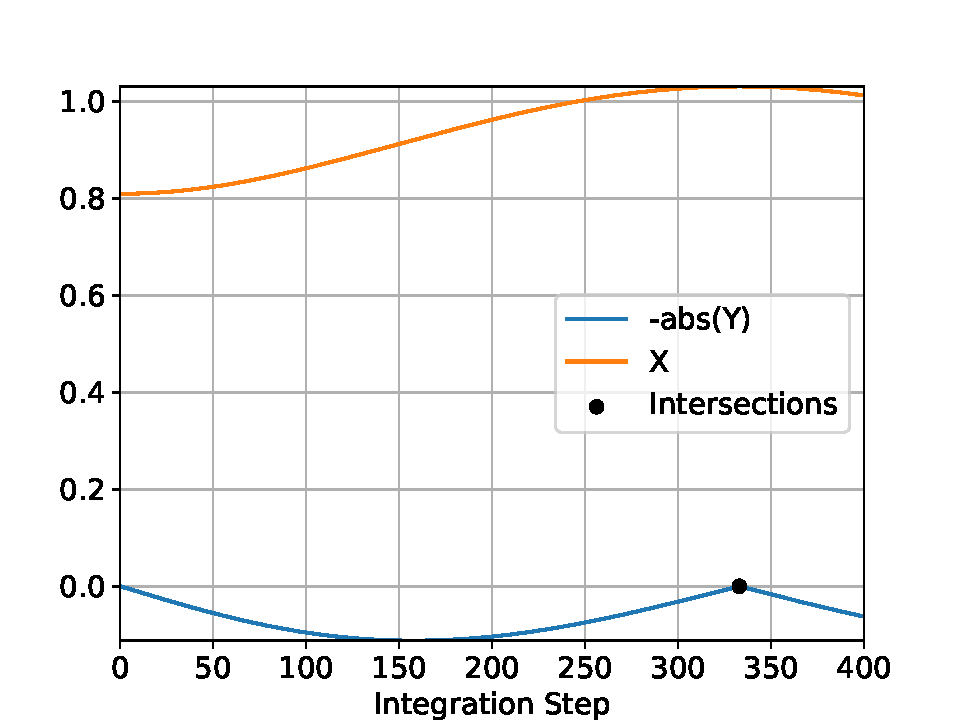
\includegraphics[width=0.7\linewidth]{figures/intersection_calculation.pdf}
    \caption{Detected intersections for the first 400 timesteps}
    \label{fig:intersection-calculation}
\end{figure}


\subsection{More Interesting Trajectories}

There were also several types of chaotic trajectories. One type was very near passes with either body, which was more likely to happen if the starting initial velocity was lower (if the starting velocity was in a direction opposite to a body) or if the satellite was closer, which likewise makes sense. 
\\
\\
\noindent
Here are 2 different chaotic trajectories that pass by the sun and the earth respectively. Both start very close and with the same small velocity.
\begin{figure}[H]
    \centering
    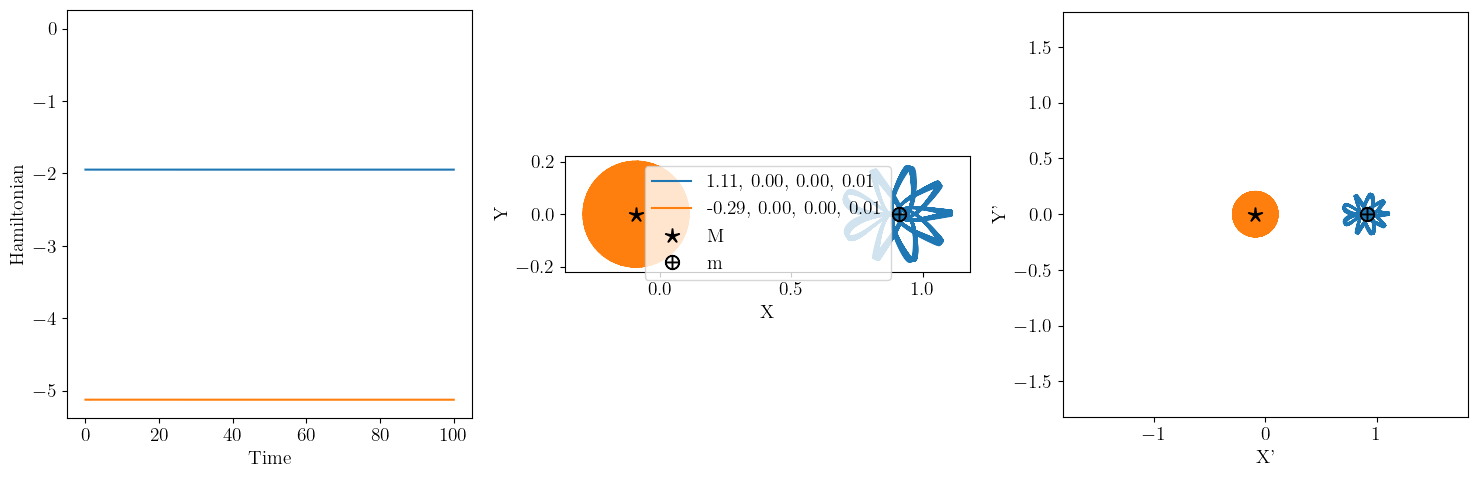
\includegraphics[width=0.7\linewidth]{figures/collision.png}
    \caption{Left: Hamiltonian over time plot of each initial condition. Middle: $m_0$ trajectories. Right: Zoomed out version of Middle}
    \label{fig:escape trajectories}
\end{figure}
\noindent
The other, more common type of chaotic motion, was the satellite spiraling out of orbit. 
\begin{figure}[H]
    \centering
    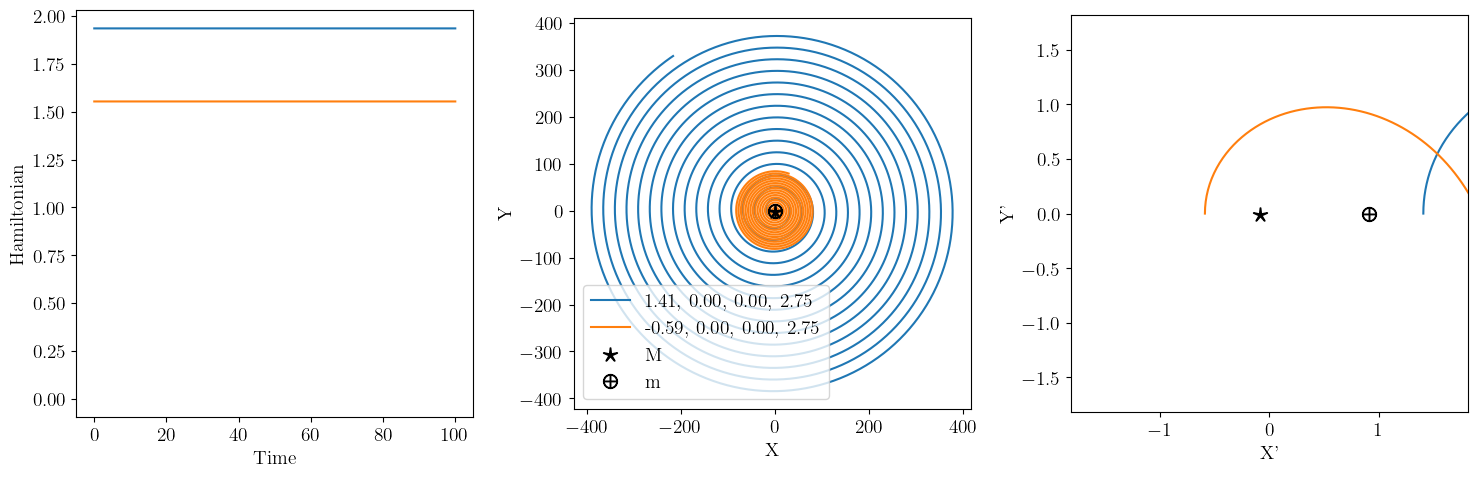
\includegraphics[width=0.7\linewidth]{figures/chaotic.png}
    \caption{Left: Hamiltonian over time plot of each initial condition. Middle: $m_0$ trajectories. Right: Zoomed in version of Middle}
    \label{fig:escape trajectories}
\end{figure}
\noindent
Figure \ref{fig:escape trajectories} shows 2 different chaotic trajectories. Both start with the same velocity and a positive hamiltonian. One starts closer to the sun, the other to the earth. Note how, though both escape orbit, the one starting closer to the earth (and thus experiencing less potential energy) spirals out faster.

\begin{figure}[H]
    \centering
    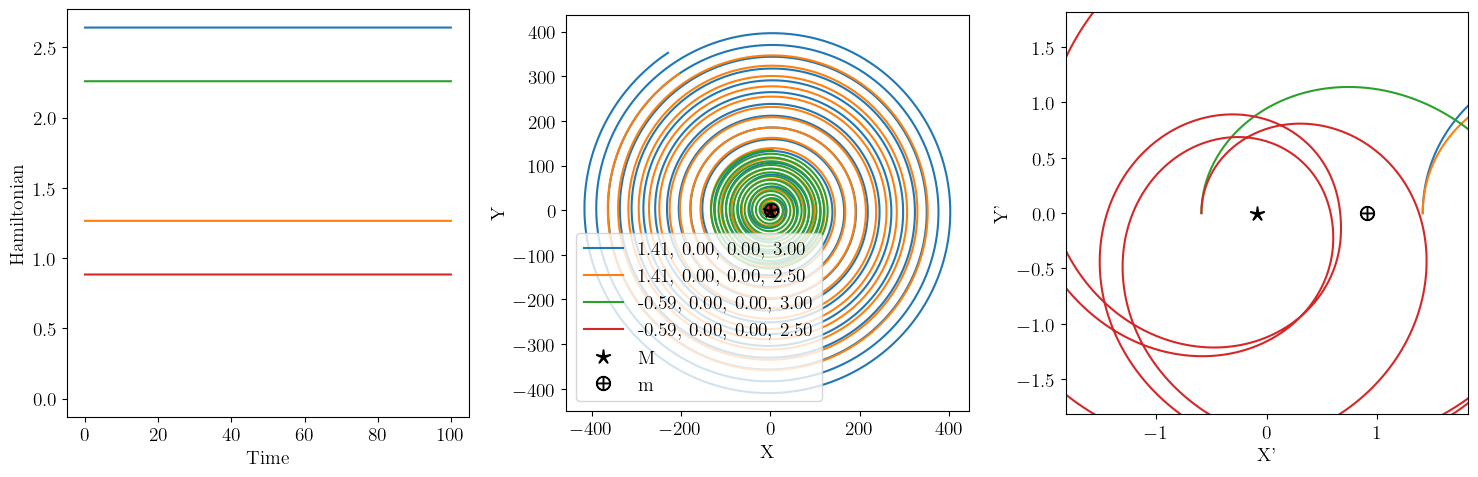
\includegraphics[width=0.7\linewidth]{figures/spiral2.png}
    \caption{Left: Hamiltonian over time plot of each initial condition. Middle: $m_0$ trajectories. Right: Zoomed in version of Middle}
    \label{fig:escape trajectories}
\end{figure}
\noindent
Figure \ref{fig:escape trajectories} shows 4 different chaotic trajectories that spiral out of orbit. Two start at the same position close to the earth, and two start at the corresponding position close to the sun. For each body, they start with two distinct velocities.
\\
\\
\noindent
We can notice that, for satellites closer to the sun than the earth that spiral out, they tend to spiral out less. Moreover, satellites with a higher starting Y' velocity (if the starting position is along the Y'-axis) tend to spiral out more. This makes sense; a higher starting velocity gives it a higher starting energy, making it more likely to escape the potential well. Starting closer to the sun also means that there is more of a pull, meaning that more energy is required to escape. 
\\
\\
\noindent
There were also some trajectories in which the satellite went between the two bodies. Here is one example:
\begin{figure}[H]
    \centering
    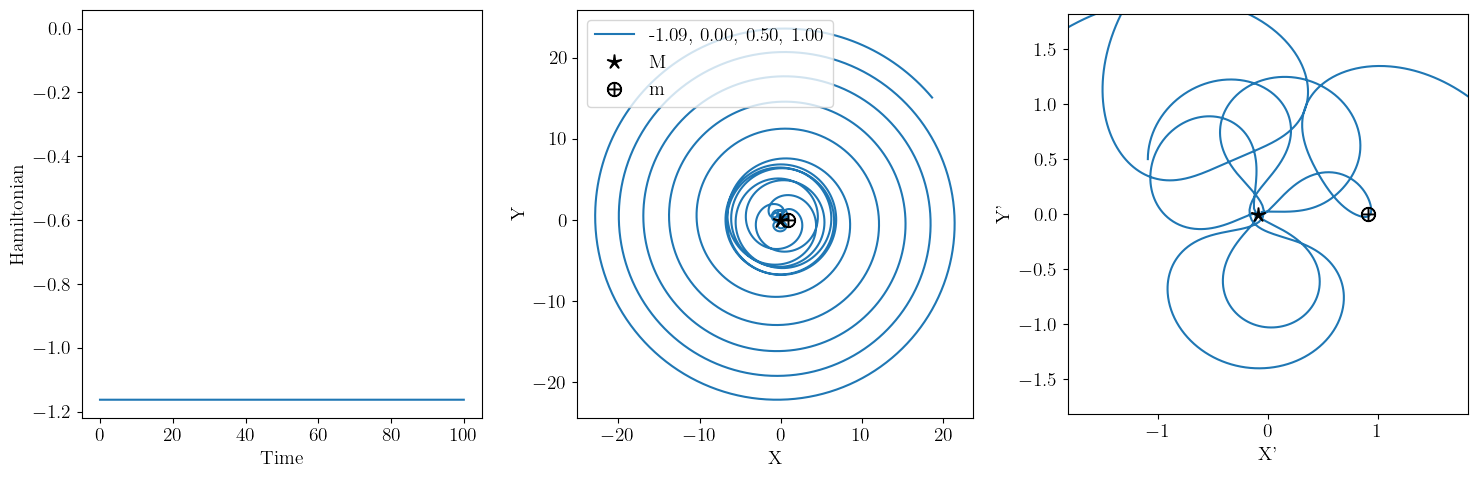
\includegraphics[width=0.7\linewidth]{figures/spiral.png}
    \caption{Left: Hamiltonian over time plot of each initial condition. Middle: $m_0$ trajectories. Right: Zoomed in version of Middle}
    \label{fig:interesting trajectories1}
\end{figure}
\noindent
Figure \ref{fig:interesting trajectories1} shows a trajectory in which the satellite starts closer to the sun, goes closer, and then goes toward the earth, and then eventually spiral out. (This probably means that, as the satellite approaches each body, it speeds up, with that extra velocity helping it escape the orbit.)
\\
\\
\noindent
A interesting demonstration of chaos is how changes in the initial conditions make large changes in the motion. 
\begin{figure}[H]
    \centering
    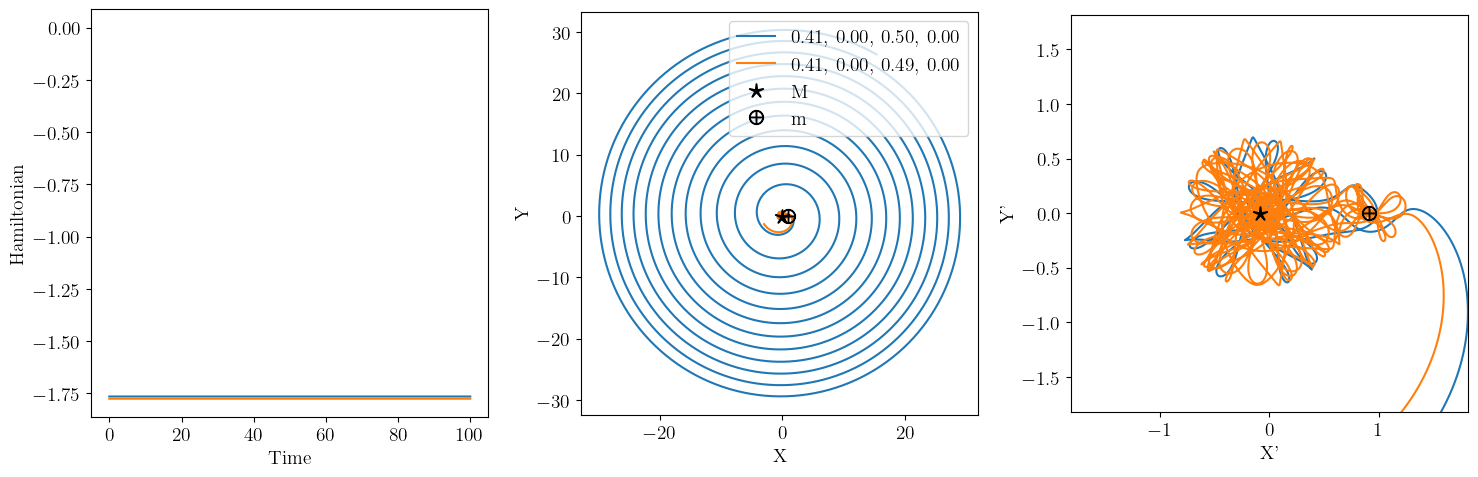
\includegraphics[width=0.7\linewidth]{figures/superchaotic.png}
    \caption{Left: Hamiltonian over time plot of each initial condition. Middle: $m_0$ trajectories. Right: Zoomed in version of Middle}
    \label{fig:interesting trajectories2}
\end{figure}
\noindent
Figure \ref{fig:interesting trajectories2} we have two statellites that start at rest with the same X'-position but very slightly different Y' positions (0.49 versus 0.5). As you can see, despite having nearly indentical hamiltonians, the satellite that is slightly farther away spirals out way more than the closer satellite.

\subsection{Lagrange Points}
Plotting some more chaotic conditions, we see an interesting phenomenon emerge:
\begin{figure}[H]
    \centering
    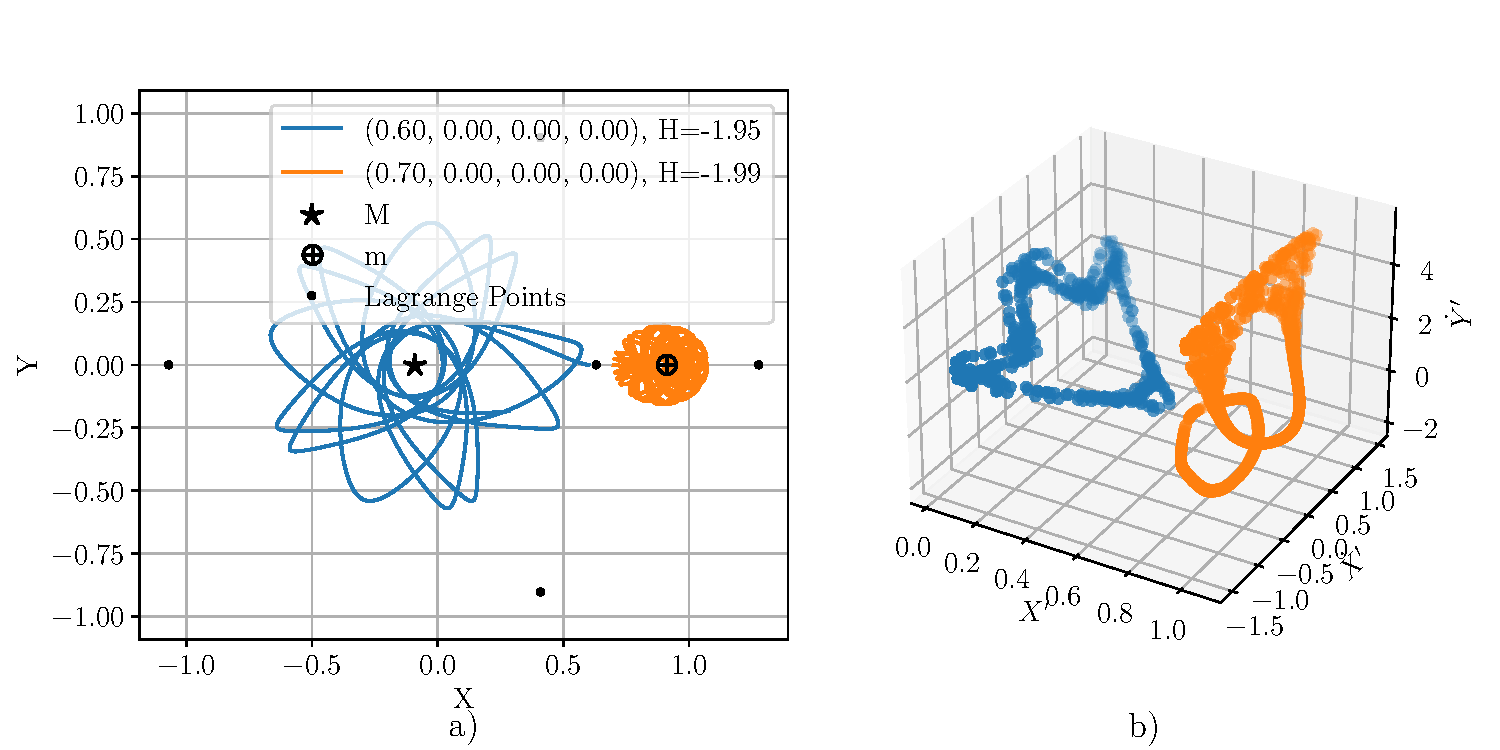
\includegraphics[width=0.9\linewidth]{figures/chaotic_investigation_orbit.pdf}
    \caption{a) Chaotic orbit trajectory for $\tau \in (0, 20)$ around $M$ and $m_\oplus$. Initial conditions listed as $(X', \dot X', Y', \dot Y')$. b) Surface of section from $\tau \in (0, 1000)$ sliced at $Y=0', X'>0$}
    \label{fig:chaotic-investigation}
\end{figure}
\noindent
It appears as though the blue trajectory around $M$ and the orange trajectory around $m_\oplus$  will meet or cross at the black point. Doing some more investigation on these points, we can see that there are actually 5 of them, and they are all equilibrium points of the system where the total force on $m_0 = 0$, or in other words critical points in the effective potential. We will investigate these critical points further. 
\\
\\
\noindent If we assume $m_0$ isn't moving, that is $\frac{\partial X'}{\partial \tau} = \frac{\partial Y'}{\partial \tau} = 0$ then the hamiltonian $h$ gives us the generalized effective potential energy $U_{eff}$ and the equations of motion if the planet isn't moving give us the generalized force $K_{eff}$ due to the effective potential energy.
\begin{align}
    U_{eff} &= - \frac{1}{2} (X'^2 + Y'^2)   - \frac{e}{\sqrt{(X'+f)^2 + Y'^2}} - \frac{d}{\sqrt{(X'-(1-f))^2 + Y'^2)}} \\
    K_{eff} &= \left|X' - \frac{d (X'-1+f)}{[(f-1+X')^2 +(Y') ^2]^{3/2}} -\frac{e (X'+f)}{[(f+X')^2 +(Y') ^2]^{3/2}}\right| \nonumber \\
    & \quad + \left|Y' - \frac{d Y'}{[(f-1+X')^2 +(Y') ^2]^{3/2}} -\frac{e Y'}{[(f+X')^2 +(Y') ^2]^{3/2}}\right|
\end{align}
This is much more clearly seen by plotting the effective potential energy, and the force on $m_0$ only due to effective potential energy as a function of $X'$ and $Y'$ as in Figure \ref{fig:lagrange-points}.
\begin{figure}[H]
    \centering
    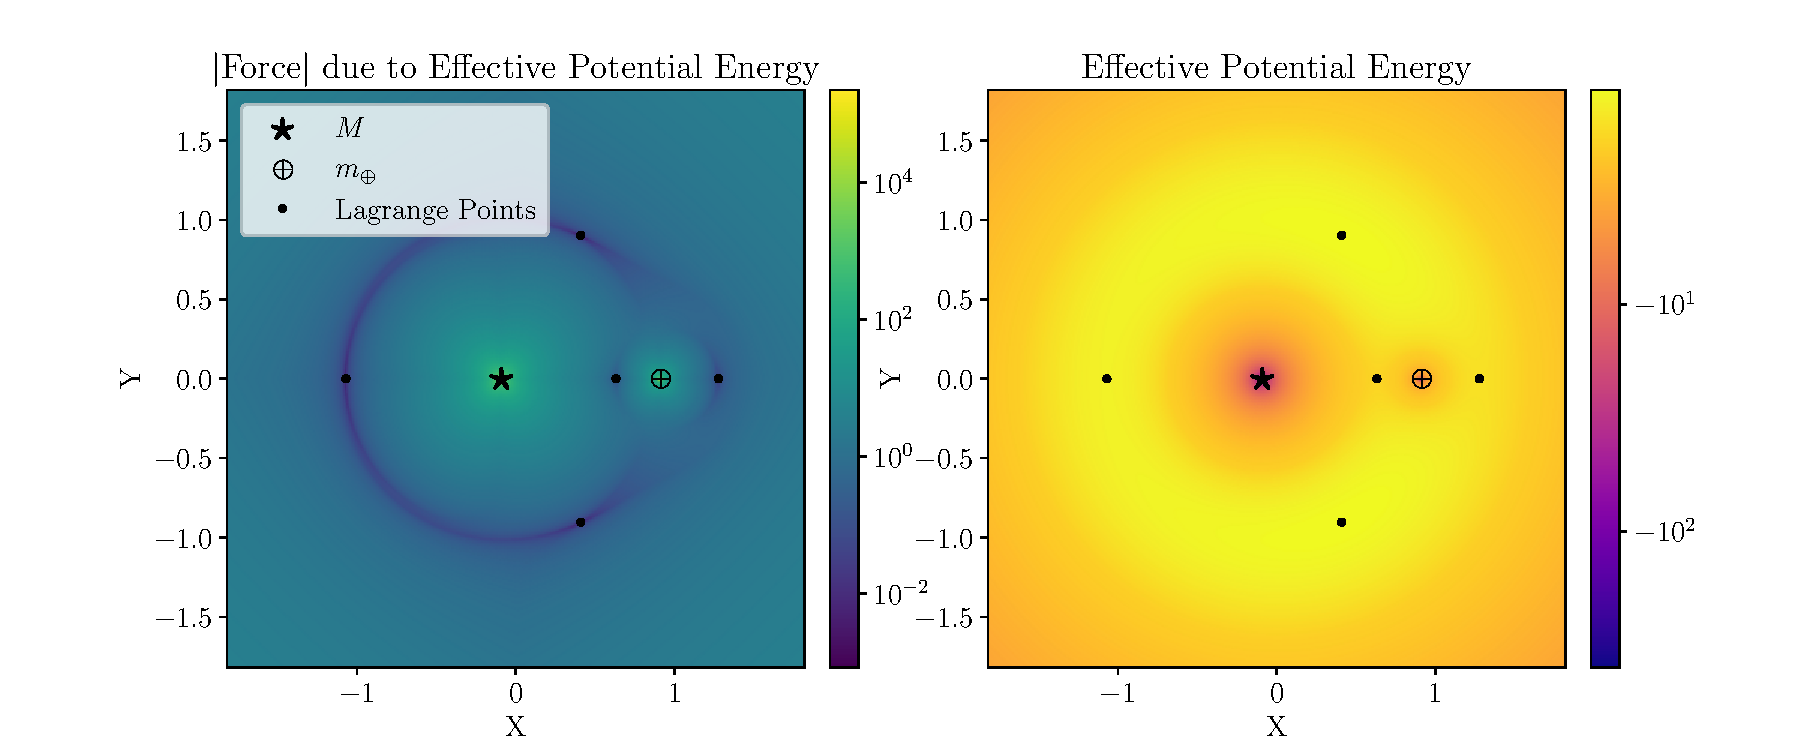
\includegraphics[width=0.9\linewidth]{figures/lagrange_points.pdf}
    \caption{Left: $K_{eff}$ versus $X',Y'$. Right: $U_{eff}$ versus $X',Y'$}
    \label{fig:lagrange-points}
\end{figure}

\begin{figure}[H]
    \centering
    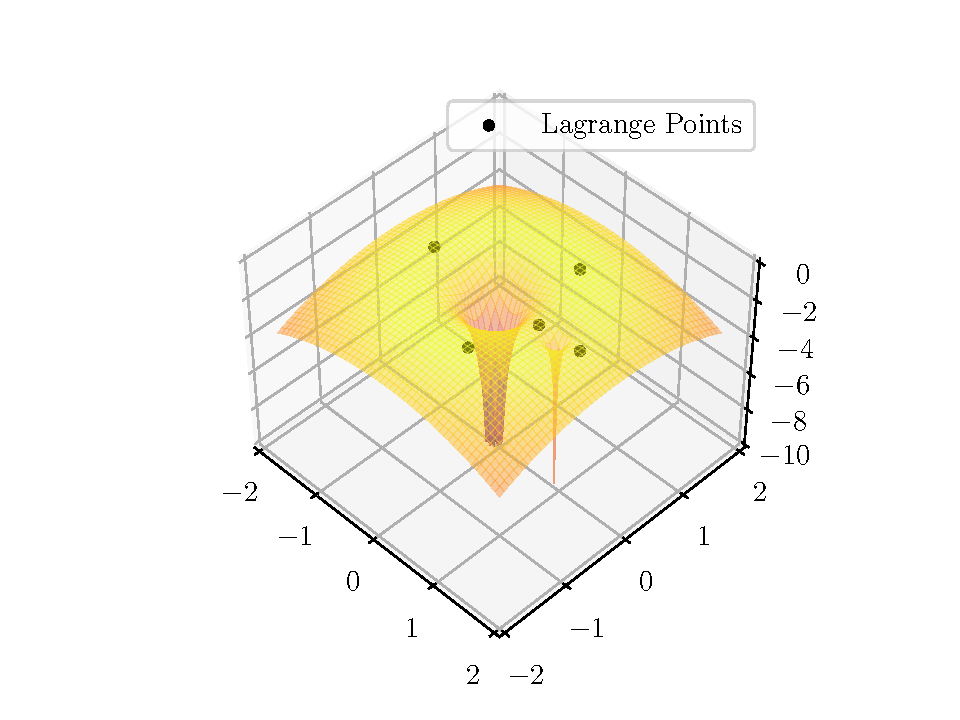
\includegraphics[width=0.8\linewidth]{figures/effective_potential.pdf}
    \caption{3D Plot of $U_{eff}$ versus $X',Y'$}
    \label{fig:Ueff}
\end{figure}

\noindent
The lagrange (or equilibrium) points are now clearly visible as minima in $K_{eff}$. As they are equilibrium points, we would expect that if $m_0$ starts exactly at one of these points it should remain there. This is (mostly) confirmed by Figure \ref{fig:lagrange-point-orbit}.
\begin{figure}[H]
    \centering
    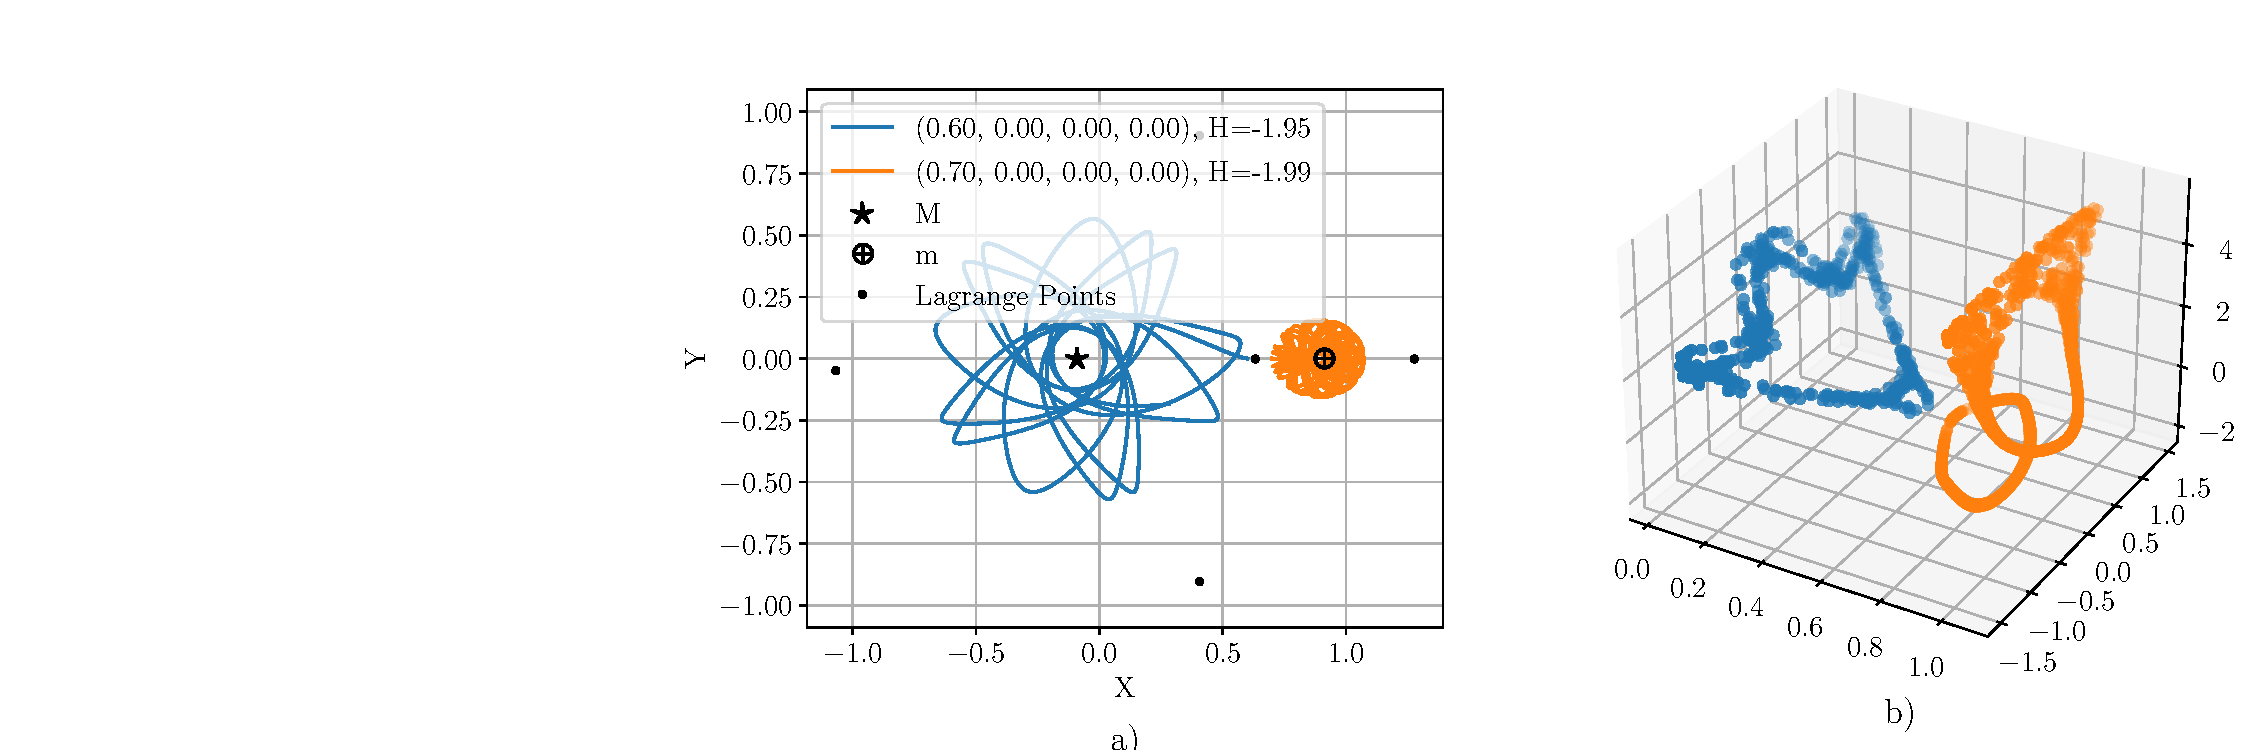
\includegraphics[width=0.6\linewidth]{figures/lagrange_point_orbit.pdf}
    \caption{Trajectory of $m_0$ starting at each lagrange point}
    \label{fig:lagrange-point-orbit}
\end{figure}
\noindent
Paths starting from 4 of the 5 lagrange points behave as desired, with the satellite stationary at those points. However, the trajectory starting at $(X', Y') = (0.63, 0)$ diverges from its lagrange point and begins to orbit $M$ due to numerical instability. From Figure \ref{fig:lagrange-points} right, we can see that all of the points are unstable, with $(0.63, 0)$ specifically being unstable and a saddle point. This makes it easy for small numerical errors in the location of the lagrange points or integration to build up and result in a diverging trajectory.
\subsection{Unreachable Locations}
Another interesting investigation sparked by Figure \ref{fig:chaotic-investigation} is the appearance that there are boundaries which $m_0$ cannot cross. From the shape of the potential $U_{eff}$, which is concave up close to $M$ and concave down on larger scales $r >> a$, where $r$ is the location of the asteroid, we expect that if $m_0$ starts close to $M$ with a low generalized energy $H=h$, it should not be able to cross the energy boundary to escape from the sun. To test this, we picked 4 energy levels and solved for initial conditions at each energy level.
\\
\\
\noindent
To simplify the solving, we restricted our search to $Y'=0, \dot X'=0, \dot Y > 0$, or, in words: trajectories that start on the $X'$ axis with no $X'$ velocity but with positive $Y'$ velocity. The majority of the trajectories generated this way are chaotic, and we will explore the full space on long enough timescales, so limiting our initial conditions does not greatly affect space we explore.  
\begin{figure}[H]
    \centering
    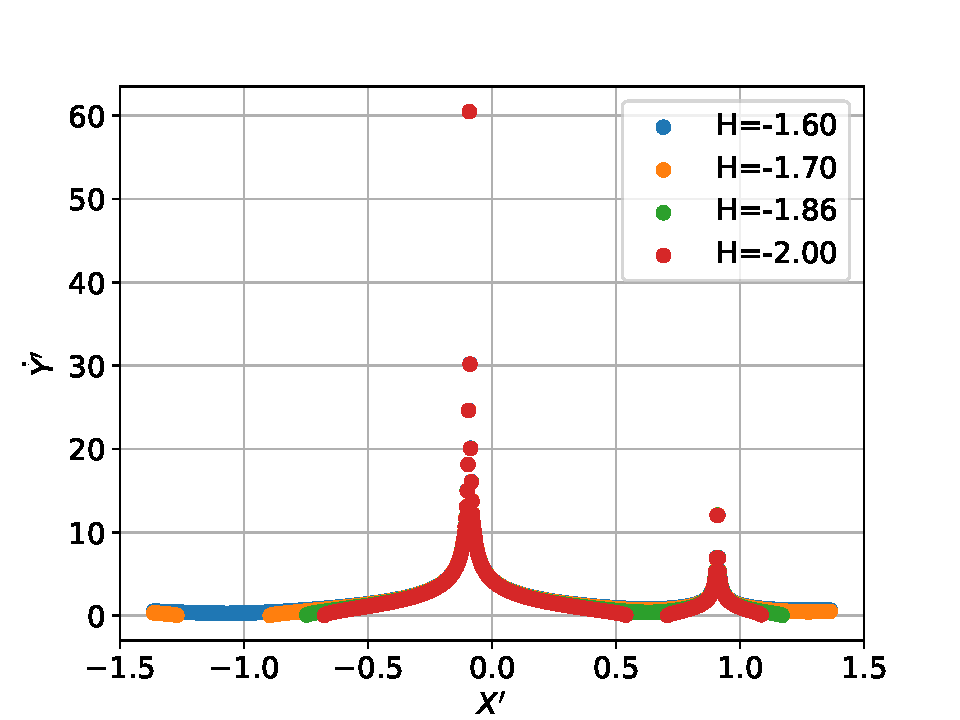
\includegraphics[width=0.7\linewidth]{figures/hamiltonian_values.pdf}
    \caption{Combinations of initial conditions with the specified generalized energy $H$. In all cases $Y'=0, \dot X'=0$}
    \label{fig:hamiltonian-values}
\end{figure}
\noindent
From the set of trajectories with each generalized energy, we selected and plotted 30 trajectories, and their surfaces of section as shown in Figures \ref{fig:hamiltonian-trajectories} and \ref{fig:hamiltonian-state-space}.
\begin{figure}[H]
    \centering
    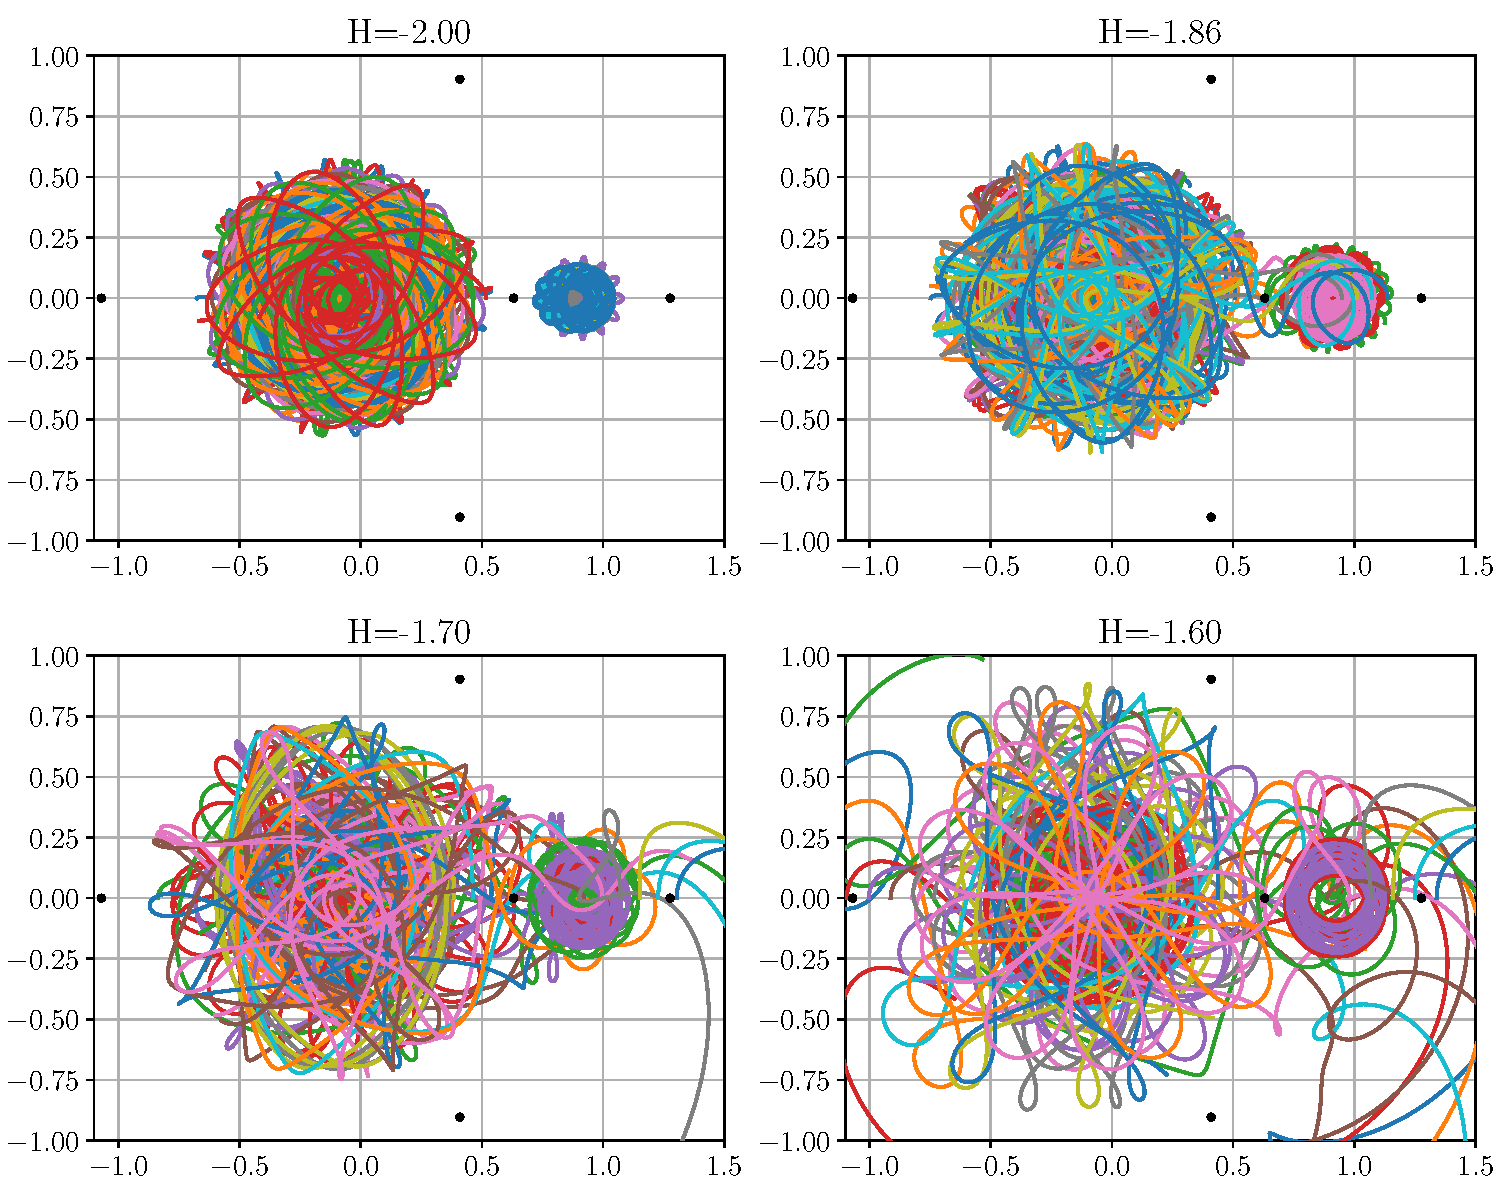
\includegraphics[width=0.6\linewidth]{figures/hamiltonian_trajectories.pdf}
    \caption{30 randomly selected trajectories from $\tau \in (0, 15)$ for each $H$ value from Figure \ref{fig:hamiltonian-values}. Grey regions indicate $U_{eff} > H$}
    \label{fig:hamiltonian-trajectories}
\end{figure}
\begin{figure}[H]
    \centering
    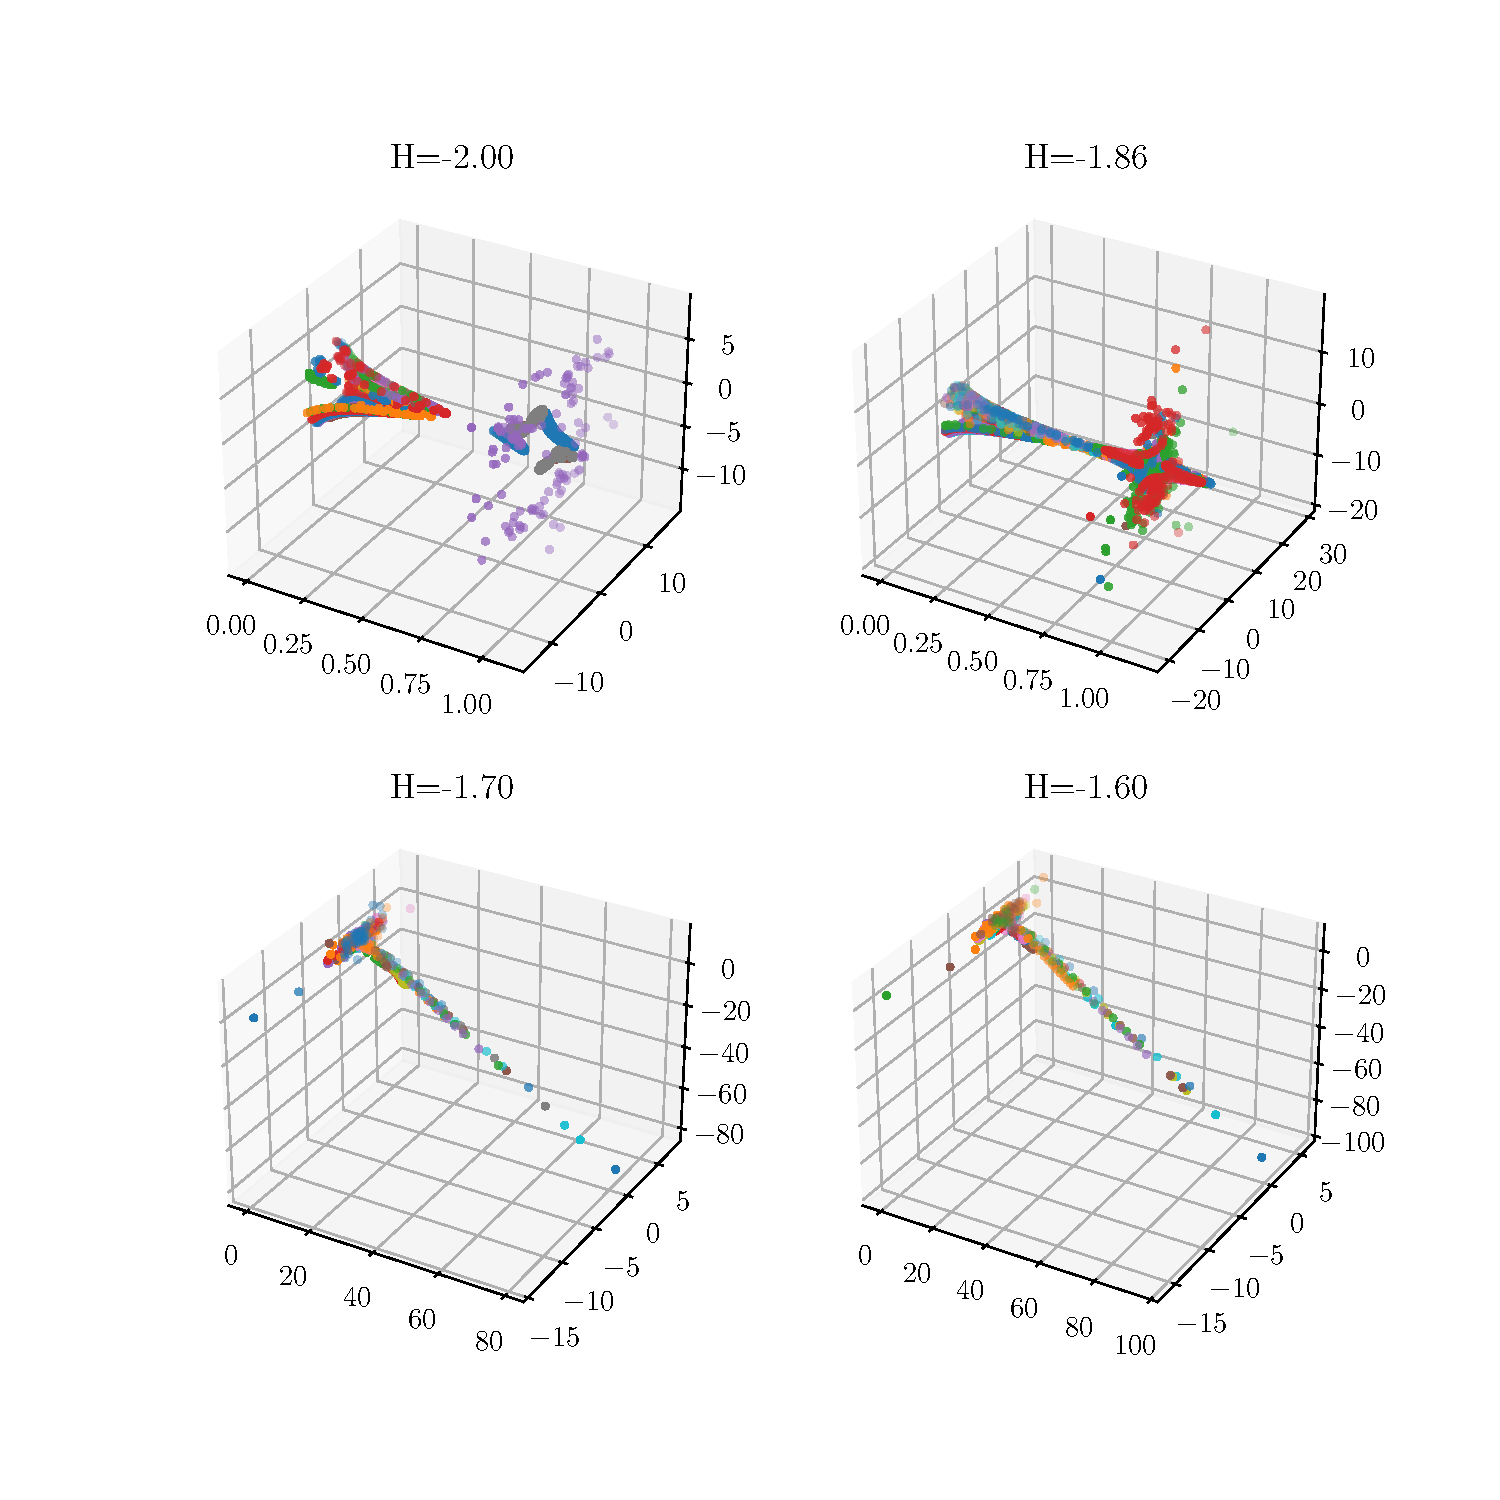
\includegraphics[width=0.6\linewidth]{figures/hamiltonian_state_space.pdf}
    \caption{Surfaces of section for Figure \ref{fig:hamiltonian-trajectories} from $\tau \in (0, 100)$ sliced at $Y=0', X'>0$}
    \label{fig:hamiltonian-state-space}
\end{figure}
\noindent
As expected, as the hamiltonian gets less negative, then there are more paths where the asteroid can escape the orbit around either body, as shown on the bottom right of Figure 15. If the Hamiltonian is smaller, though, the asteroid will only have a trajectories in which it orbits either the sun or the earth, but it cannot cross between the bodies, as shown on the top left of Figure 15. 
\\
\\
\noindent
In the plot we see that none of the trajectories can cross into regions of higher energy than where they started! At lower energies we also observe interesting behavior where $m_\oplus$ almost acts as a gateway for $m_0$ to enter, lowering the potential energy barrier relative to other locations around $M$. In other words, it's easier for a satellite to approach the sun if it starts the same distance away in the side where the earth is in between them versus not.
% \\
% \\
% Now, we explore some initial conditions. First, let the earth be the actual earth and the sun the actual sun. Then, to an order of magnitude, we get:

% \begin{equation}
%     m_\oplus=10^{24} kg
% \end{equation}
% \begin{equation}
%     M=10^{30} kg
% \end{equation}
% \begin{equation}
%     a=10^{11} m
% \end{equation}
% \begin{equation}
%     G=10^{-12} \frac{m^3}{kg*s^2}
% \end{equation}
% Omega is one over a full orbit from the earth to the sun, so, to an order of magnitude, we get: 
% \begin{equation}
%     \Omega=10^{-7}s
% \end{equation}

% Then, we...graph over a range of different h values? Any intuition for what'd be normal, here? 

% Also, like, what about where the asteroid starts? Does that matter? 

% The next thing to think about is initial conditons.... Hm. It'd be cool to think about some other real-world systems (like jupiter or earth-moon-satellite), but I feel like they'd be pretty similar. It could be interesting to see how far we have to push things to start getting chaotic solutions, tho....
% It'd also be interesting to see, like, if the asteroid can collide with the planet. 

% To find other interesting initial conditions, we try to graph the state space plot of X versus $\dot X$. To do this, we solve for Y in terms of X using the equation for h, our nondimensionalized Hamiltonian. We get: 
% (SOMETHING)

% If you look at the scale of the h-axis, you can see that it's pretty much constant, as it should be! 

% Using this to plot the state space, we get: 


\section{Summary and Conclusion}
\label{sec:summary and conclusion}

From the planar circular-restricted three-body problem, we explored several different conditions. The stable configurations tended to be closer to either the sun or the earth, and, in these configurations, the asteroid orbited either the sun or the earth, as expected. When put farther away from either the sun or the earth and with lower initial velocities, the asteroid tends to spiral away from both bodies in chaotic motion. Moreover, if put too close to either body, the asteroid ends up falling into either the earth or the sun. 
\\
\\
\noindent
We also explored the lagrange points of the system. To do this, we plotted where the force on the asteroid was smallest, indicating where there were minimima in the potential energy function. If put at these these points, the asteroid would stay still, rotating with the earth and the sun. However, if put even slightly closer to one or the other, the asteroid would follow the other and have a drastically different path! 
\\
\\
\noindent
Finally, we looked at the uncrossable boundaries given certain values for the hamiltonian. More specifically, we looked at paths between the earth and the sun where the asteroid crossed between the earth and the sun with only vertical speed. As the hamiltonian gets higher, then more paths are allowed, and more of those paths are chaotic. 
\\
\\
\noindent
In the future, it would be interesting to characterize more of the chaotic paths that end up going between the sun and the earth and to do a more in-depth exploration of how changing each initial condition changes the trajectoriy. It would also be cool to look at changing the parameters to model those of the real earth and sun and to model other such systems.
\\
\\
\noindent
The full code and figures are available at: \\
\url{https://github.com/kavidey/PHYS111/blob/main/computational_project/computational_project.ipynb}


% \section{Misc Fun Facts that we should probably cut}
% \label{sec:Misc Fun Facts that we should probably cut}
% Apparently some guy proved that the infinite power series of the 3 body problem converges! But it's not that useful bc there's like 10 to the power of 8000000 terms 

% Hm, apparently you can also prove that you can't have a triple collision in the ordinary 3 body problem

% Apparently the planar restriction comes bc you can show mathematically that, if you start in a plane, you stay there, but I couldn't really follow the proof. 

% Apparently the sun-earth-moon system is chaotic but has a narrow stability range? Not sure what that means 


\end{document}